\documentclass{article}

% Required for inserting images
\usepackage{graphicx}

% to have more colors avelable
\usepackage{xcolor}

% to insert hiperlinks
\usepackage[colorlinks=true,linkcolor=cyan]{hyperref}

% to have better references
\usepackage[noabbrev]{cleveref}

% to use prefix for references
\usepackage{etoolbox}

% to set the margin of the page
\usepackage[a4paper, total={6.5in, 9in}]{geometry}

% to make indentations
\usepackage{changepage}

% for sub figures
\usepackage{subcaption}

% to allow putting description text to te side of an image
\usepackage{wrapfig}

% rule for reference to fugures
\pretocmd{\thefigure}{F}{}{}

% settings for how to indend the page when neaded
\newenvironment{indented_section}
  {\adjustwidth{3em}{0pt}}
  {\endadjustwidth}

\title{Use Of Jigsaw Puzzle Solving Algorithms In The Real World}
\author{Luca Sartore}
\date{May 2023}

\begin{document}

\maketitle

\newpage

% make the table of content without the hiperlink color
{
  \hypersetup{linkcolor=black}
  \tableofcontents
}

\newpage

\section{Abstract}
The jigsaw puzzle problem has been in the eye of computer scientists for a while,
and some clever solutions have already been found. These algorithms are made to
work with a “digital” jigsaw puzzle~\ref{fig:figure_digital_puzzle},
but there aren't papers (at least not popular enough to be searchable)
that try to apply the solution
to a “real world” jigsaw puzzle~\ref{fig:figure_real_puzzle}.\newline
The problem has been tackled by some small projects. But, as said earlier,
the process and eventual challenges has never been documented by a full paper,
this wants to be the first.\newline
As a bonus the paper will also cover the creation of a user friendly app
that will be open source and free to use.

\section{Introduction}
\subsection{Classification}
This paper will focus on type 2 puzzles. A type 2 puzzle is a puzzle where the position, and the orientation of each piece is unknown. 
\subsection{Digital vs Real-World Jigsaw Puzzles}

There is  another important distinction between different types of puzzles.
They can be divided into “digital” and “real world” jigsaw puzzles.
\label{document:DigitalVSReal}

% figure of digital jigsaw puzzle    
\begin{figure}[h]
    \caption{An example of a “digital” jigsaw  puzzle}\label{fig:figure_digital_puzzle}
    \centering
    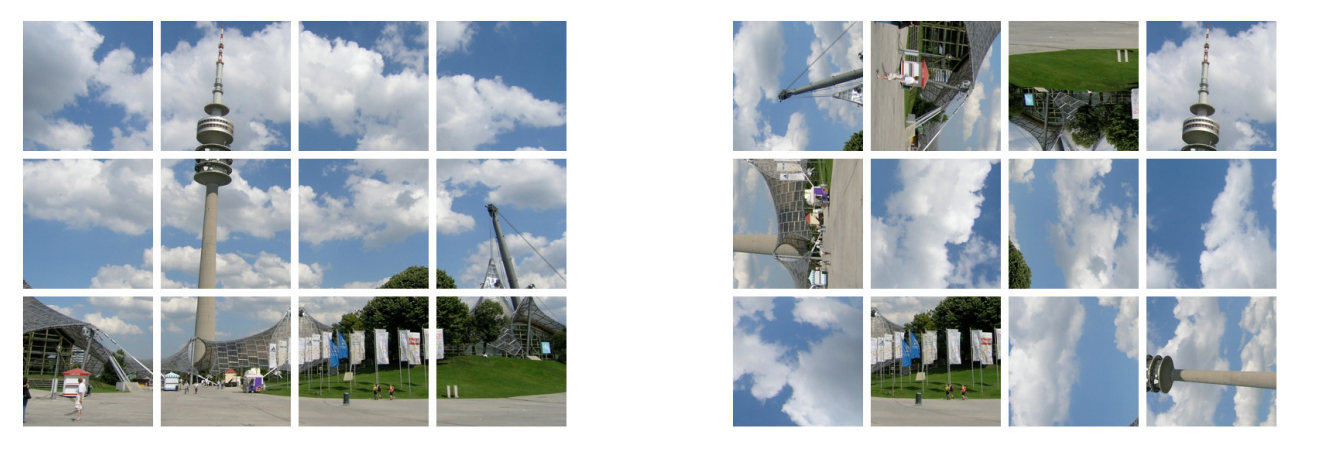
\includegraphics[height=0.25\textwidth]{pictures/digital_puzzle.png}
\end{figure}

% figure of real jigsaw puzzle    
\begin{figure}[h]
    \caption{An example of a “real world” jigsaw  puzzle}\label{fig:figure_real_puzzle}
    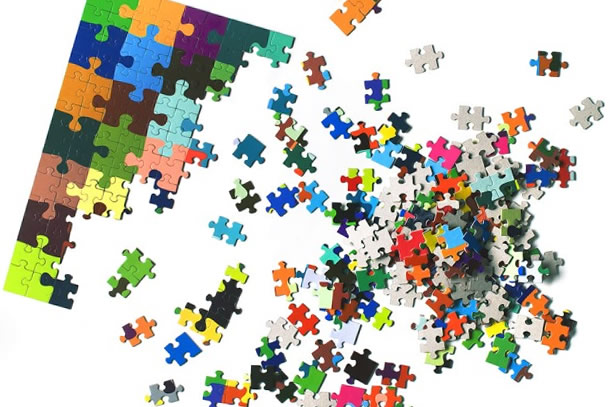
\includegraphics[height=0.25\textwidth]{pictures/real_puzzle.jpg}
    \centering

\end{figure}

The reason this distinction is important is because,
despite the generic concept of the puzzle not changing,
obtaining accurate matches of a piece's characteristics
is far easier with a digital puzzle,
since there are far less things that can go wrong.


% figure of a mesurement error
\begin{figure}[h]
    \caption{An example of what can go wrong when dealing with the real world}\label{fig:figure_measurement_error}
    
\includegraphics[height=0.25\textwidth]{pictures/example_bad_piece.jpg}
    \centering
\end{figure}

\section{Previous Literature}
This section will analyze 3 different algorithms that have been proposed
as a solution of type 2 puzzles. The objective is to understand the
strengths and the weaknesses of each one, to build up some knowledge
that will be useful for the next section.

\subsection{General Structure Of The Algorithms}

All the algorithms that will be analyzed are composed of 3 sub algorithms:


\begin{indented_section}

    \subsubsection{The Splitter:} This component takes as input one or more images
    containing all the pieces. It then split all the pieces from each other,
    9and split each piece into his four sides.\label{document:splitter}

    \subsubsection{The Comparator:} This component compares each side with all the
    others, in order to understand whether they match or not.\newline
    There are two distinct kinds of “Comparator” algorithms:
    The “Binary Comparison” and the “Non Binary Comparison”.
    As the name suggests when comparing two sides with a “Binary Comparison”
    the result can either be 0 (they do not match) or 1 (they match).
    In contrast a “Non Binary Comparison” can give any value between 0 and 1.
    This allows states of uncertainty to be represented.\label{document:comparator}

    \subsubsection{The Solver:} This component  uses the information provided by the
    Comparator~\ref{document:comparator}, and tries to find a solution
    (i.e.\ a position and an orientation for each piece)
    that is the most likely to be correct.\label{document:solver}

\end{indented_section}

\subsection{Solving Jigsaw Puzzles By The Graph Connection Laplacian~\cite{GCL}}
This algorithm falls in the “binary comparison” category~\ref{document:comparator}.
And can be used to understand the strength and weaknesses
of this approach.\newline
The main benefit of this approach is speed,  having a binary comparison allows
some specific optimization, in particular the use of some graph theory techniques.\newline
The  algorithm has a time complexity of ruffly \(O(N^2)\). Which is in line with the theoretical
minimum for jigsaw puzzle solving, according to the study:
“No easy puzzles: Hardness results for jigsaw puzzles~\cite{ON2Claim}”.\newline
The negative aspect might be the accuracy, since by using only two states
(match or not match) some informations are lost, compared to a non binary comparison.
To quantify accuracy the paper used the “neighbors comparison” metric,
which “calculates the percentage of pairs of image patches that are matched correctly”.\newline
\label{document:GCL}


\subsection{A Genetic Algorithm-Based Solver for Very Large Jigsaw Puzzles~\cite{GA}}
This paper applies a genetic algorithm to the jigsaw puzzle problem, with some promising results.\newline
The algorithm seems to have a \(O(N^2)\) time complexity, with time slightly lower than the previous example
(But it is impossible to know for sure which one is faster, given that they didn't specify the hardware used).\newline
The paper has used the same method to evaluate accuracy that the previous one used
(neighbors comparison) so it is easy to compare them.\newline
The algorithm falls in the “Non binary comparison”~\ref{document:comparator};
this should give it an advantage, since it has more data to work with.\newline
Unfortunately this advantage does not compensate for the worst precision
of the algorithm itself, and the accuracy results are equivalent,
if not slightly worse than the previous algorithm.\newline
It is important to keep in mind that for the very nature of genetic algorithms,
it might be possible that the accuracy would have been better if they had allowed
it to run for more generations.\newline
\label{document:GA}

\subsection{Computer Vision Powers Automatic Jigsaw Puzzle Solver~\cite{Abto}}
The solutions~\ref{document:GCL} and~\ref{document:GA} can be considered “state of the art” for digital jigsaw puzzles.
But, as already introduced in section~\ref{document:DigitalVSReal} and better explained in section TODO,
appalling the solution to the real world can be challenging.\newline
This solution is possibly a “state of the art” for real world puzzles.\newline
In reality calling this a “solution” is incorrect,
since all it does is find the best 8 matches and asks the user which one to place.
Making the algorithm not autonomous.\newline
Even ignoring this major detail, making an analysis of this solution has proven to be challenging,
since the article is more of a publicity stunt than an academic paper.
In fact, the code is not open source and the information about the time needed to solve the puzzle is missing.\newline
The article only shows a single puzzle solved, with a 9$\times$6 dimension.\newline
Even with all of these problems this article still is one of the best example of a solution for real world puzzle.

\section{The Objective Of This Paper}
After reading some of the previous literature for this problem, some conclusions could be drawn:
The problem of “digital jigsaw puzzle” has been solved many times, and is already well optimized.\newline
On the other hand, the problem of “real world jigsaw puzzle” has mostly been ignored\newline
by the academic community.\newline

The objective of this paper is to fill this void, by answering the following questions:
\begin{itemize}
    \item Can the current state of the art solutions for digital puzzles be used for real world puzzles, or the unpredictable nature of real world data makes it impossible?
    \item If the algorithms cannot be applied to the real world, what is a possible solution that is more redundant to imprecise data?

  \end{itemize}

\section{The Setup}

To answer these questions, some data to start with,
and an algorithm to analyze the data; in particular the necessary components are:


\subsection{The Puzzle To Solve}

The first step is finding a real world puzzle to solve;
It has been decided to use a classic 500 piece puzzle, and use a printer's
scanner to digitize the pieces.\newline
The puzzle has been scanned in various sub-sizes to allow the testing of different configurations. 
A resolution of 1200 ppi has been used to ensure a sharp and precise image
of the piece, as seen in image~\ref{fig:figure_measurement_error}.
The puzzle has been scanned backward, since the comparator algorithm
that has been used REF does not use colors,
and having an uniform color would make splitting the pieces easier.

\subsection{Splitting The Pieces}
As introduced in section~\ref{document:splitter}, the first step to solve a puzzle
is to split an image composed of many pieces into individual ones.
This is relatively straightforward, and can be done with the following steps:

\begin{itemize}
  \item Apply a threshold and transform an RGB image into a binary mask.
  \item Find all individual Blobs
  (a Blob is just set of connected pixels with the same color) and for each one:

  \begin{itemize}
  \item Calculate the area (the number of pixels the Blob is made of)

  \item Add it to the set of pieces only if his area in within a certain range (to avoid small pieces of dust ending up counted as pieces)

  \end{itemize}

\end{itemize}

\subsection{Splitting The Sides}

The next step following the general template~\ref{document:splitter}
is to split a pieces into
his 4 sides, this could be done with the following steps:

\begin{itemize}

  \item \textbf{Remove the holes from the piece:}\newline
  To do so the program computes the convex hull of the piece~\ref{fig:s_s_ch},
  then calculates the difference between the convex hull and the original image,
  and obtains an image with the “filler areas”~\ref{fig:fig:s_s_og_minus_ch}.
  These filler areas have very different shapes,
  depending on what has generated them (a “hole” or a “knob” in the piece).
  So they can be classified, and added to the original piece only if
  they are generated by a hole, obtaining an image without holes~\ref{fig:s_s_no_holes}.

  \item \textbf{Remove the knobs from he piece}\newline
  To do so the image without holes gets eroded~\ref{fig:s_s_erosion} and then dilated~\ref{fig:s_s_dilatation}.
  This generates an image that resembles the original one, but has no knobs.
  Then the program finds the pixels that are white in the image without holes,
  but not in the image that has been eroded and dilated.
  This generates a set of Blobs~\ref{fig:s_s_no_holes_minus_expansion},
  but again, the shape of the blob is very different depending on what has generated it
  (an “angle” or a “knob”), so they can be classified.
  Then the program removes from the image with no holes all the pixels that are
  close to a Blob generated by a knob, obtaining an image without knobs and holes~\ref{fig:s_s_no_knobs}.
  
  \item \textbf{Find the coordinates of the four corners}\newline
  To find the coordinates of the corners, the program uses a tree steps approximation.
  It initially finds the minimum enclosing rectangle,
  and uses the coordinates of the corners of the rectangle
  as first approximation~\ref{fig:s_s_min_enc_rec}.\newline
  As a second approximation it takes,
  from the white pixels that are close to the first approximation,
  the pixel that has the most black pixels within a certain distance.
  Then it considers only the pixels that are within a certain
  distance of the second approximation, and finds the minimum
  enclosing triangle of sed pixels~\ref{fig:s_s_min_enc_triangle}.\newline
  The corner of the triangle that is closest to the second
  approximation is the third and final approximation
  of the corner of the piece.
  The position of the four corners can be seen in image~\ref{fig:s_s_corners_found}.

  \item \textbf{Split each side using the previously found coordinates.}\newline
	Once the program has found the four coordinates of the corners, to obtain each
  side. An example of a single side can be seen in image~\ref{fig:s_s_a_piece_side}.
\end{itemize}

\begin{figure}
  \begin{subfigure}{0.3\textwidth}
    \centering
    
\includegraphics[width=\linewidth]{pictures/original_piece.jpeg}
    \caption{Original binary mask of a piece.}
    \label{fig:s_s_og}
  \end{subfigure}
  \hfill
  \begin{subfigure}{0.3\textwidth}
    \centering
    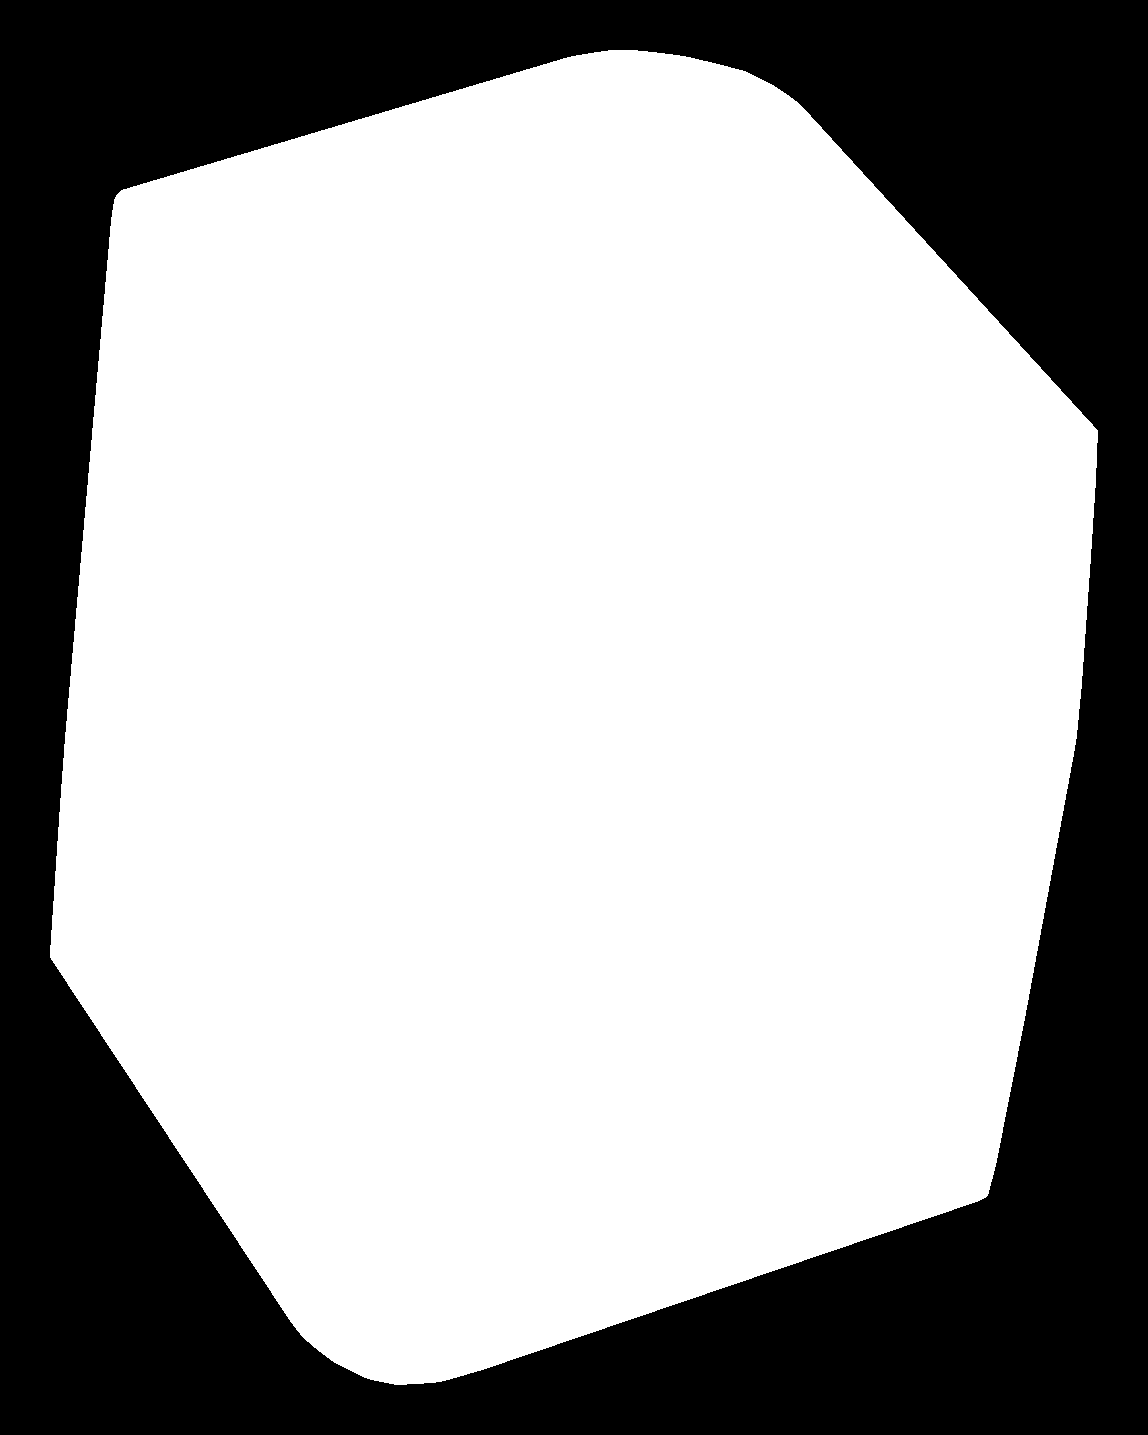
\includegraphics[width=\linewidth]{pictures/remove_holes_convex_hull.png}
    \caption{Convex Hull of a piece.}
    \label{fig:s_s_ch}
  \end{subfigure}
  \hfill
  \begin{subfigure}{0.3\textwidth}
    \centering
    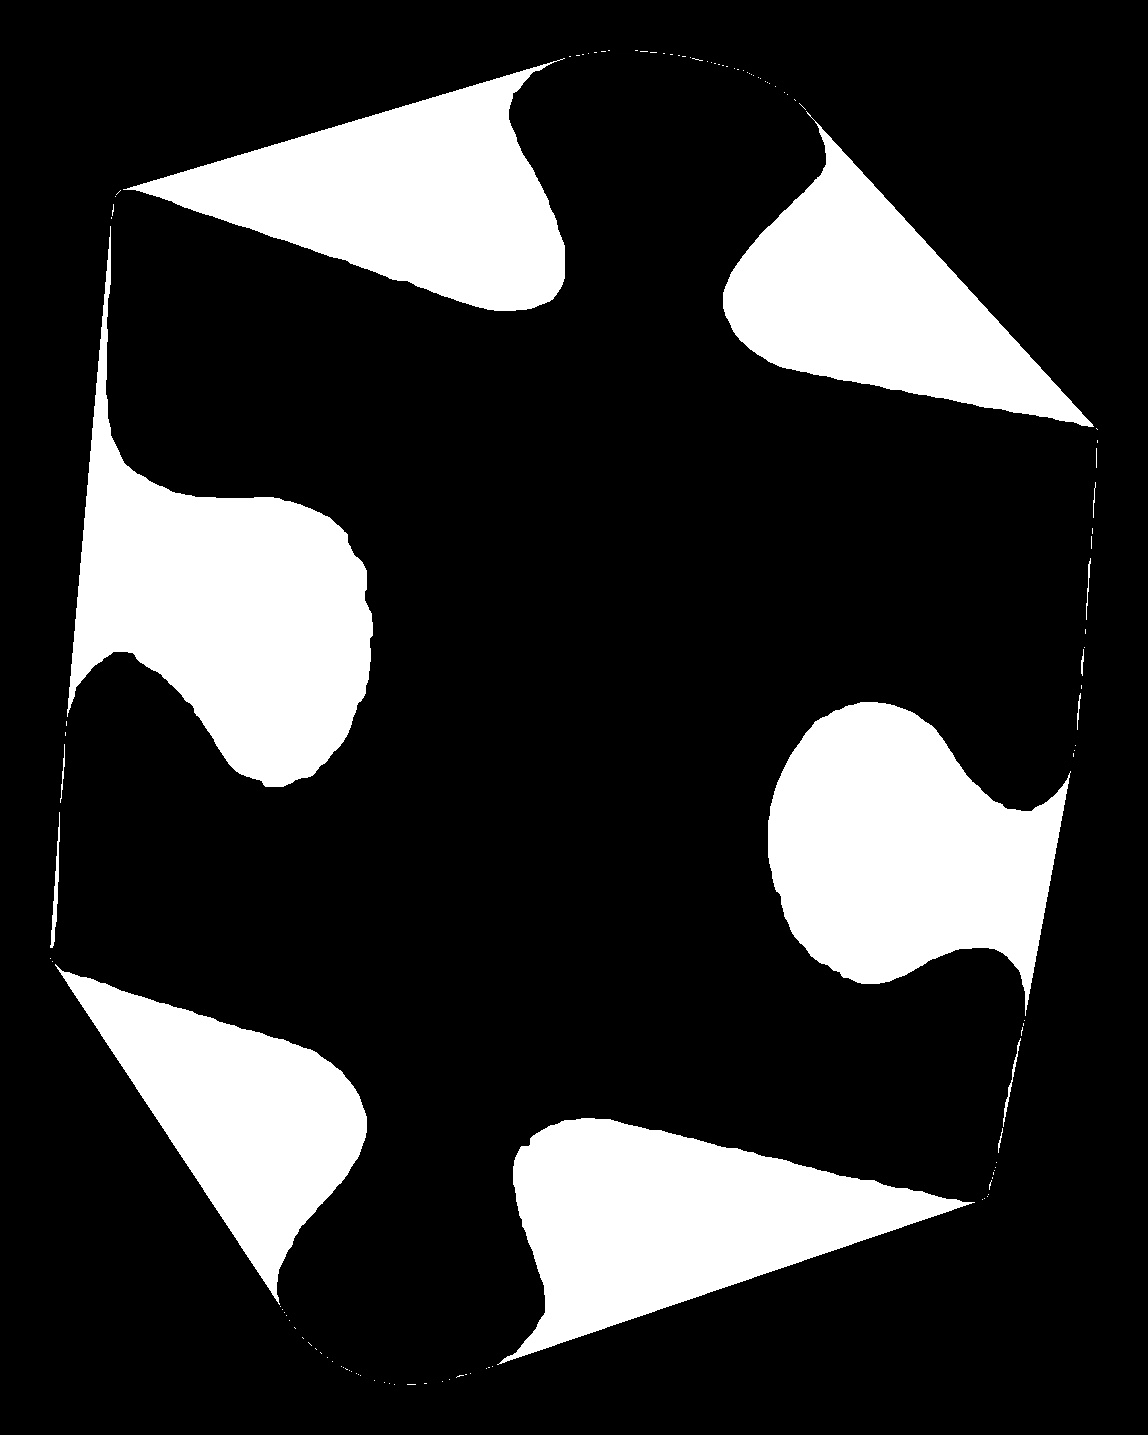
\includegraphics[width=\linewidth]{pictures/remove_holes_filler_areas.png}
    \caption{Difference:~\ref{fig:s_s_ch} \textminus~\ref{fig:s_s_og}.}
    \label{fig:fig:s_s_og_minus_ch}
  \end{subfigure}
  \vspace{1cm}
  \begin{subfigure}{0.3\textwidth}
    \centering
    
\includegraphics[width=\linewidth]{pictures/piece_with_no_hole.png}
    \caption{Piece~\ref{fig:s_s_og} with holes removed.}
    \label{fig:s_s_no_holes}
  \end{subfigure}
  \hfill
  \begin{subfigure}{0.3\textwidth}
    \centering
    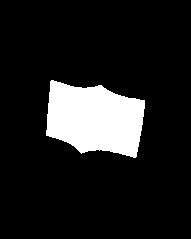
\includegraphics[width=\linewidth]{pictures/remove_knobs_erosion.png}
    \caption{Mask~\ref{fig:s_s_no_holes} eroded.}
    \label{fig:s_s_erosion}
  \end{subfigure}
  \hfill
  \begin{subfigure}{0.3\textwidth}
    \centering
    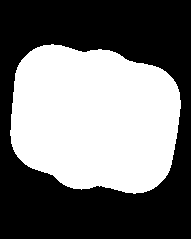
\includegraphics[width=\linewidth]{pictures/remove_knobs_expansion.png}
    \caption{Mask~\ref{fig:s_s_erosion} dilated.}
    \label{fig:s_s_dilatation}
  \end{subfigure}
  \vspace{1cm}
  \begin{subfigure}{0.3\textwidth}
    \centering
    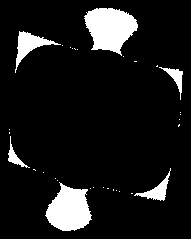
\includegraphics[width=\linewidth]{pictures/remove_knobs_knob_pixels.png}
    \caption{Difference:~\ref{fig:s_s_no_holes} \textminus~\ref{fig:s_s_erosion}.}
    \label{fig:s_s_no_holes_minus_expansion}
  \end{subfigure}
  \hfill
  \begin{subfigure}{0.3\textwidth}
    \centering
    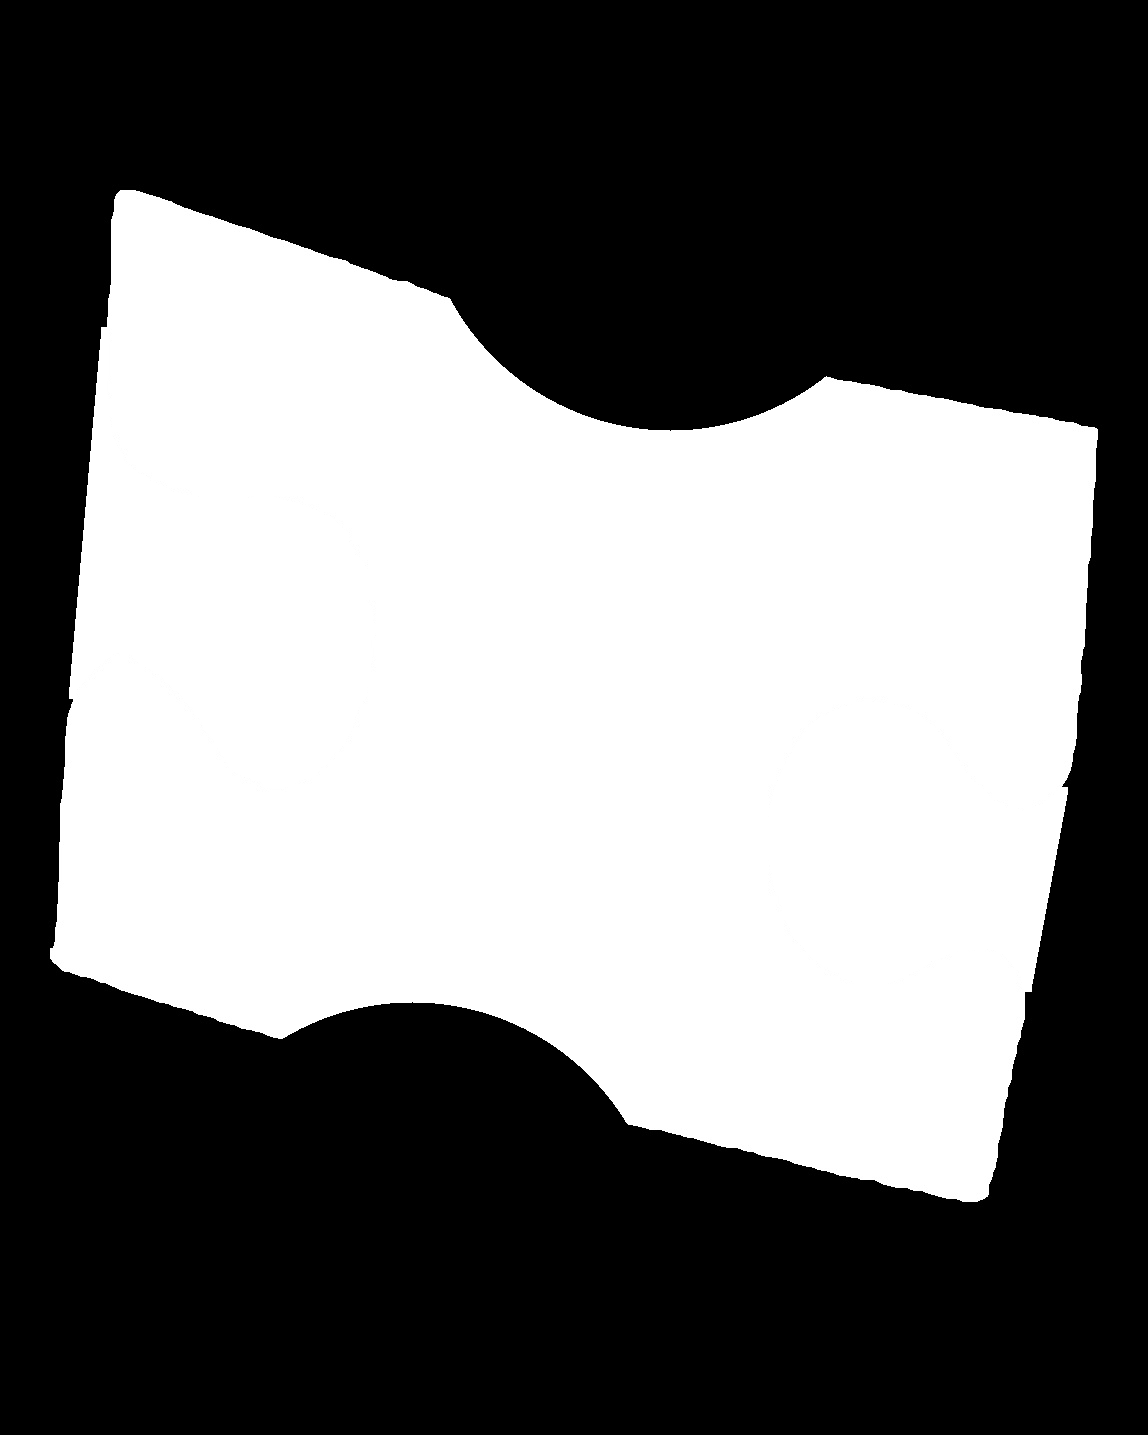
\includegraphics[width=\linewidth]{pictures/piece_with_no_knobs.png}
    \caption{Piece~\ref{fig:s_s_no_holes} with knobs removed.}
    \label{fig:s_s_no_knobs}
  \end{subfigure}
  \hfill
  \begin{subfigure}{0.3\textwidth}
    \centering
    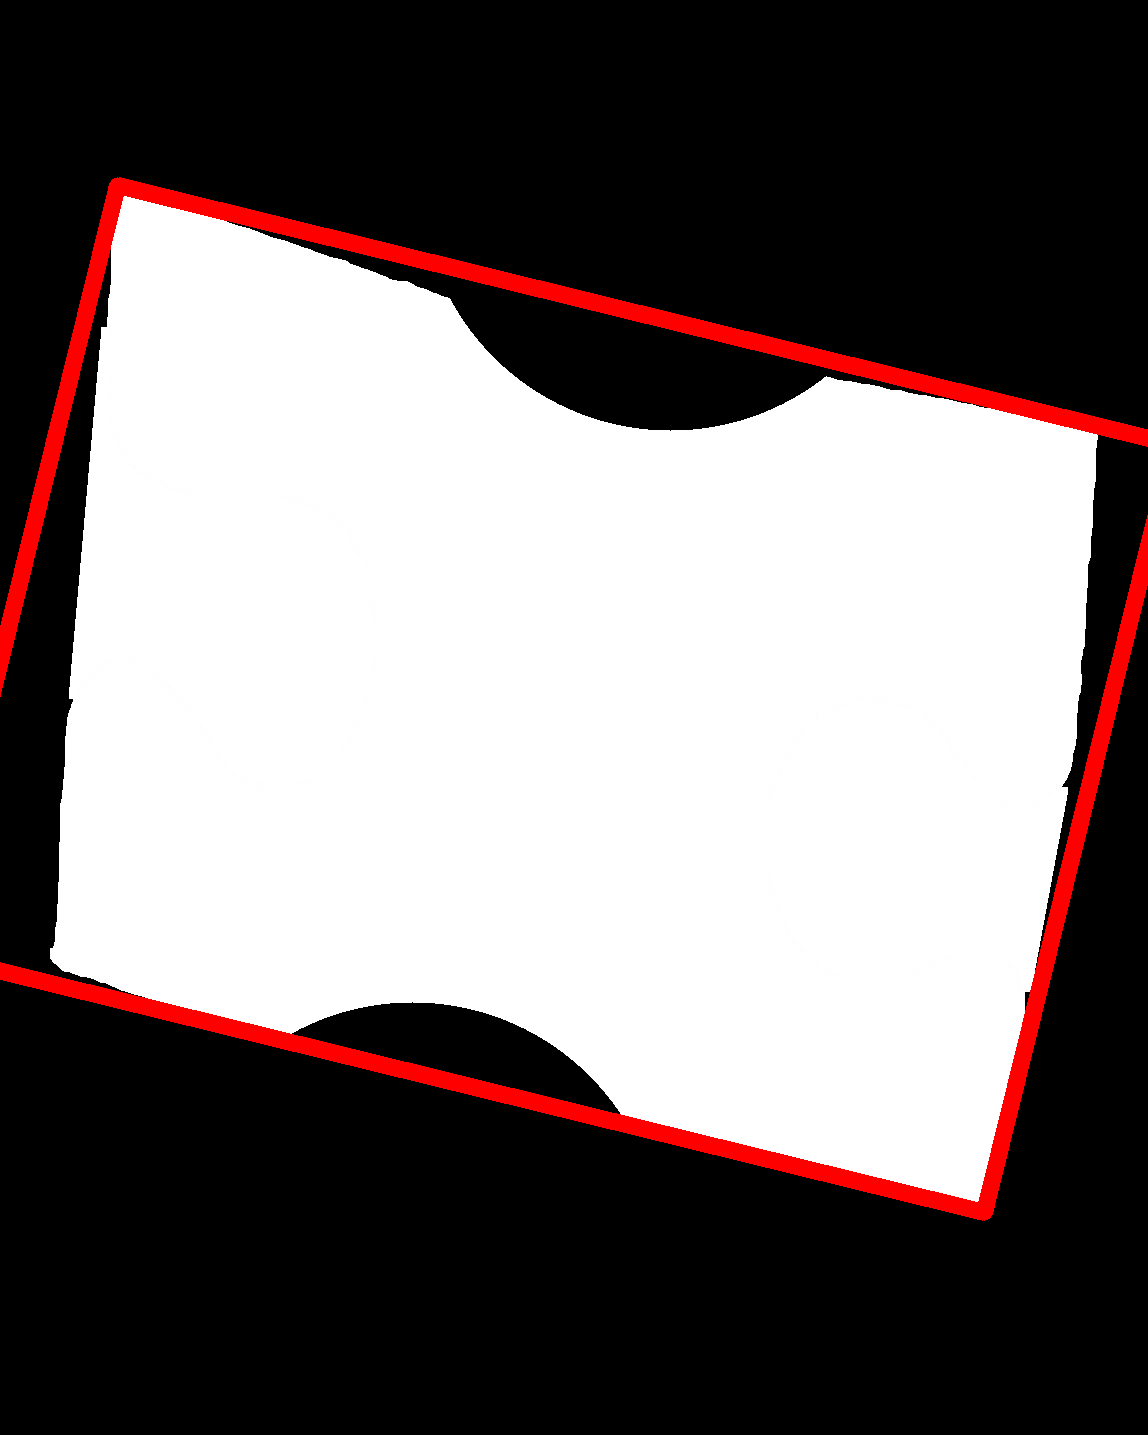
\includegraphics[width=\linewidth]{pictures/find_corners_min_enclosing_rectangle.png}
    \caption{Min enclosing rectangle of~\ref{fig:s_s_no_knobs}.}
    \label{fig:s_s_min_enc_rec}
  \end{subfigure}
\end{figure}
\clearpage
\begin{figure}\ContinuedFloat
  \begin{subfigure}{0.3\textwidth}
    \centering
    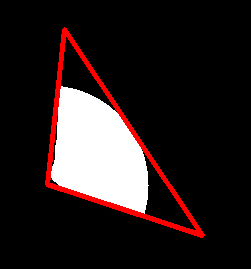
\includegraphics[width=\linewidth]{pictures/find_corners_min_enclosing_triangle.png}
    \caption{Min enclosing triangle of the bottom right corner of~\ref{fig:s_s_no_knobs}.}
    \label{fig:s_s_min_enc_triangle}
  \end{subfigure}
  \hfill
  \begin{subfigure}{0.3\textwidth}
    \centering
    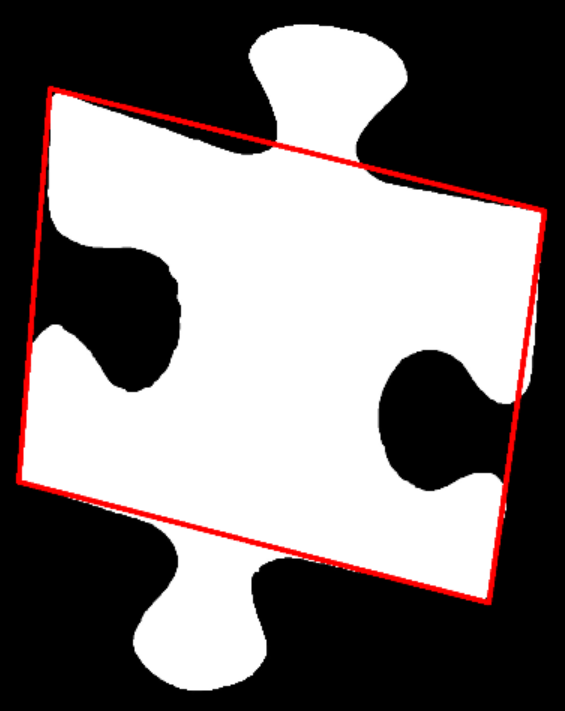
\includegraphics[width=\linewidth]{pictures/corners_found.png}
    \caption{The corners of the piece~\ref{fig:s_s_og}.}
    \label{fig:s_s_corners_found}
  \end{subfigure}
  \hfill
  \begin{subfigure}{0.3\textwidth}
    \centering
    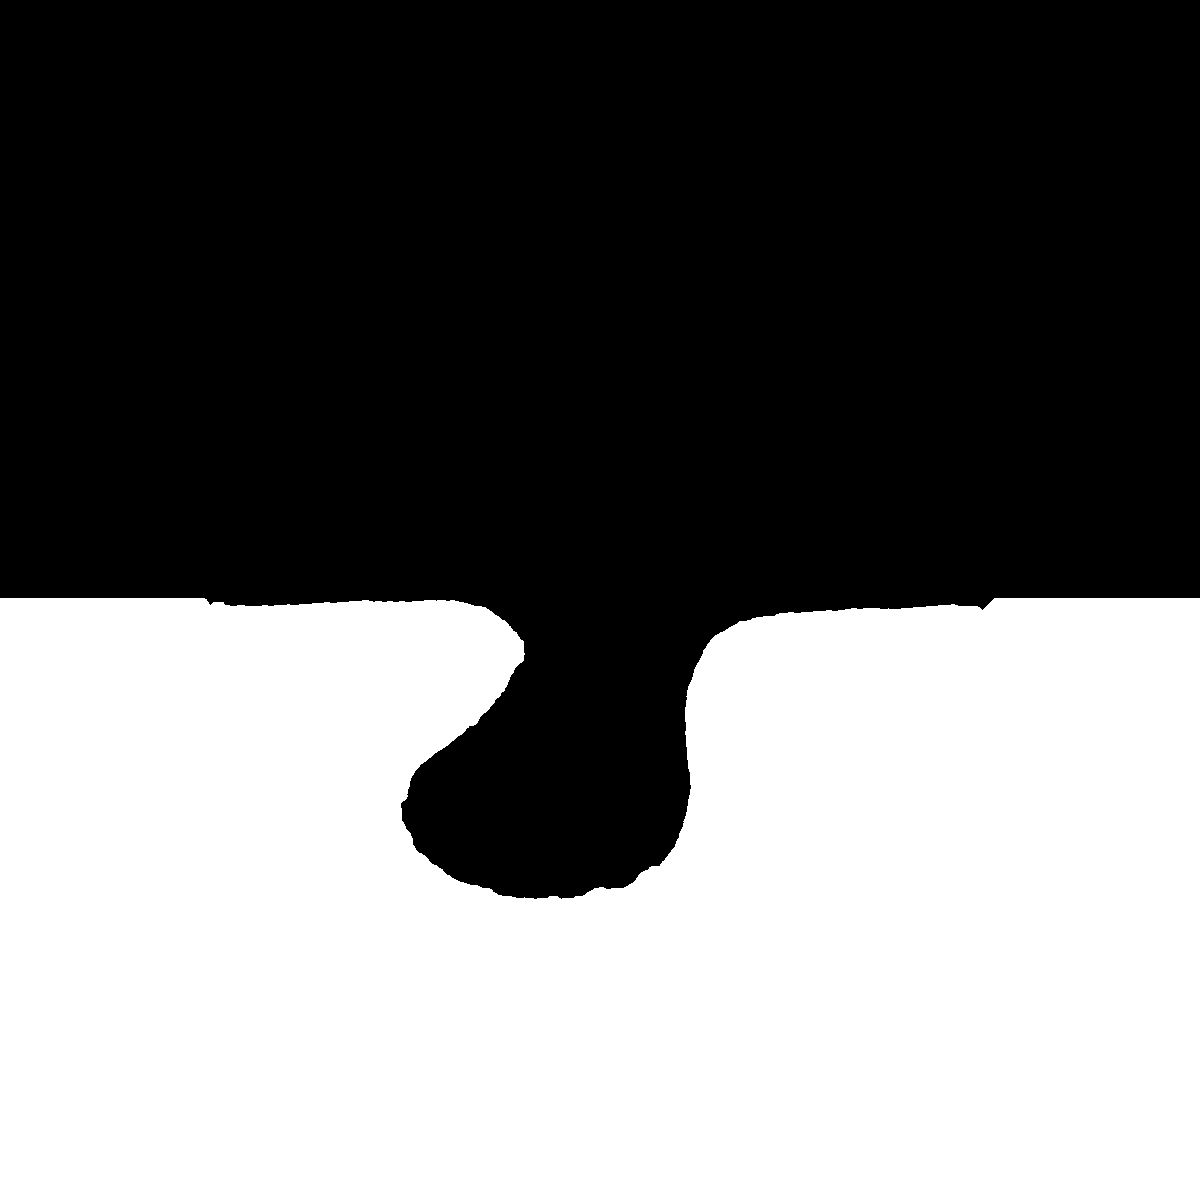
\includegraphics[width=\linewidth]{pictures/piece_side.png}
    \caption{One of the sides of the piece~\ref{fig:s_s_og}.}
    \label{fig:s_s_a_piece_side}
  \end{subfigure}
  
  \caption{Steps needed to split an image into his four sides.}
  \label{fig:splitting_sides}
  
\end{figure}

\subsection{Comparing the sides}
The last step needed before it is possible to start working on
a solver algorithm, is to compare the sides that have been
generated by the previous step.\newline
In order to generate a compatibility shore,
the program compute the following steps:

\begin{itemize}
  \item For each side, it considers only the border, and it makes the border thicker.
  \item It puts two sides attached to each other using the coordinates of the corners (In the same way a human would do to test if two pieces fit together).
  \item It calculates the “Or Area”; that is, the number of pixels that belong to the border of one side or the other.
  \item It calculates the “And Area”; that is, the number of pixels that belong to the border of both sides.
  \item It calculates the final shore, which is defined as: \(Shore = \frac{And \space Area}{Or \space Area}\), and goes from 0 to 1.
\end{itemize}


\begin{figure}[htbp]
  \centering
  \begin{minipage}[t]{0.44\textwidth}
    \vspace{3pt} % Ensure alignment of the top of the minipage
    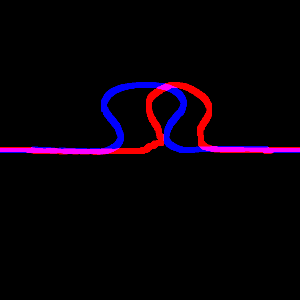
\includegraphics[width=\textwidth]{pictures/side_comparation.png}
  \end{minipage}
  \hfill
  \begin{minipage}[t]{0.54\textwidth}
    \caption{\newline
    In this image we can see two sides that have been
    compared, one side is drowned in red, the other one in blue.
    In this picture, the “Or Area” is represented by all non
    black pixels; The “And Area” is represented by all the
    purple pixels.}
  \end{minipage}
\end{figure}
\clearpage

\section{bo}

% referneces page
\clearpage
\begin{thebibliography}{9}

  %Graph Connection Laplacian
  \bibitem{GCL}
    Vahan Huroyan, Gilad   Lerman and Hau-Tieng Wu,
    Solving Jigsaw Puzzles By The Graph Connection Laplacian,
    2020.
    \url{https://arxiv.org/pdf/1811.03188.pdf}.
  % Genetic algorighm
  \bibitem{GA}
    Dror Sholomon, Omid David and Nathan S. Netanyahu,
    A Genetic Algorithm-Based Solver for Very Large Jigsaw Puzzles,
    2013.
    \url{https://openaccess.thecvf.com/content_cvpr_2013/papers/Sholomon_A_Genetic_Algorithm-Based_2013_CVPR_paper.pdf}.
  
    % Claim of best solution O(N^2)
  \bibitem{ON2Claim}
    Michael Brand,
    No easy puzzles: Hardness results for jigsaw puzzles,
    2015.
    \url{https://www.sciencedirect.com/science/article/pii/S0304397515001607}.

    % abtosoftware real world solution
  \bibitem{Abto}
    AbtoSoftware,
    Computer Vision Powers Automatic Jigsaw Puzzle Solver,
    2019.
    \url{https://www.abtosoftware.com/blog/computer-vision-powers-automatic-jigsaw-puzzle-solver}.
  
\end{thebibliography}

\end{document}
